
\documentclass[12pt,a4paper]{article}

% ------------------------------------------------------------
% Fonts & layout
% ------------------------------------------------------------
\usepackage[T1]{fontenc}
\usepackage[utf8]{inputenc}
\usepackage{lmodern}
\usepackage{microtype}
\usepackage{geometry}
\geometry{margin=1in}
\usepackage{array}
\usepackage{booktabs}
\usepackage[table]{xcolor}
\usepackage{tikz}
\usetikzlibrary{positioning}

% ------------------------------------------------------------
% Math
% ------------------------------------------------------------
\usepackage{amsmath,amssymb,amsthm,mathtools}

% Standard operators
\DeclareMathOperator{\id}{id}
\DeclareMathOperator{\im}{im}
\DeclareMathOperator{\coker}{coker}
\DeclareMathOperator{\Hom}{Hom}

\DeclareMathOperator{\Spec}{Spec}
\DeclareMathOperator{\Proj}{Proj}

% Categories / notation
\newcommand{\Ab}{\mathbf{Ab}}
\newcommand{\PreSh}{\mathbf{PreSh}}
\newcommand{\Sh}{\mathbf{Sh}}

\newcommand{\F}{\mathcal F}


% basic number sets
\newcommand{\RR}{\mathbb{R}}

% sheaf letters

\newcommand{\G}{\mathcal G}

\newcommand{\GG}{\mathbb G}


\newcommand{\AffSch}{\mathbf{AffSch}}
\newcommand{\ZZ}{\mathbb Z}

\newcommand{\PP}{\mathbb P}

\usepackage{tikz}
\usetikzlibrary{decorations.pathreplacing}
\usetikzlibrary{positioning,arrows.meta}

% sheaf of continuous real-valued functions
\newcommand{\Czero}{\mathcal C^0}        % “C^0”
\newcommand{\CzeroX}{\mathcal C^0_X}     % sheaf on X (optional)

\newcommand{\Cinfty}{\mathcal C^\infty}
\newcommand{\CinftyM}{\mathcal C^\infty_M} % if you use C^\infty_M

% number sets / standard symbols
\newcommand{\CC}{\mathbb{C}}

% structure sheaf notation in complex geometry
\newcommand{\OO}{\mathcal{O}}
\newcommand{\OOX}{\mathcal{O}_X} % optional convenience



\newcommand{\Sch}{\mathrm{Sch}}
\newcommand{\Rings}{\mathrm{Rings}}

\newcommand{\kappares}{\kappa}
\newcommand{\GammaX}{\Gamma(X,\mathcal O_X)}

\newtheorem{theorem}{Theorem}[section]
\newtheorem{proposition}[theorem]{Proposition}
\newtheorem{lemma}[theorem]{Lemma}

\newcommand{\nilrad}{\sqrt{(0)}}

\newcommand{\Frac}{\operatorname{Frac}}
\newcommand{\codim}{\operatorname{codim}}
\newcommand{\trdeg}{\operatorname{trdeg}}

\newcommand{\height}{\operatorname{height}}

\newcommand{\Pic}{\operatorname{Pic}}
\newcommand{\divisor}{\operatorname{div}}

\newcommand{\Z}{\mathbb{Z}}
\newcommand{\Cl}{\operatorname{Cl}}

\providecommand{\Spec}{\operatorname{Spec}}
\providecommand{\A}{\mathbb A}
\providecommand{\Pj}{\mathbb P}
\providecommand{\G}{\mathbb G}

% ------------------------------------------------------------
% Links
% ------------------------------------------------------------
\usepackage{xcolor}
\usepackage{hyperref}
\usepackage{bookmark}
\hypersetup{
  colorlinks=true,
  linkcolor=blue!50!black,
  urlcolor=blue!50!black,
  citecolor=blue!50!black,
  pdftitle={Algebraic Geometry 18
  },
  pdfauthor={},
  pdfsubject={Lecture notes (reorganized)},
  pdfcreator={TeXStudio / LaTeX}
}

% ------------------------------------------------------------
% Diagrams
% ------------------------------------------------------------
\usepackage{tikz-cd}

% ------------------------------------------------------------
% Lists
% ------------------------------------------------------------
\usepackage{enumitem}
\setlist[itemize]{topsep=4pt,itemsep=2pt,parsep=0pt,partopsep=0pt}
\setlist[enumerate]{topsep=4pt,itemsep=2pt,parsep=0pt,partopsep=0pt}

% ------------------------------------------------------------
% Theorem environments
% ------------------------------------------------------------
\newtheoremstyle{notespace}{6pt}{6pt}{\normalfont}{}{\bfseries}{.}{0.5em}{}
\theoremstyle{notespace}
\newtheorem{definition}{Definition}[subsection]

\newtheorem{corollary}[definition]{Corollary}
\newtheorem{remark}[definition]{Remark}
\newtheorem{example}[definition]{Example}
\newtheorem{warning}[definition]{Warning}


\DeclareMathOperator{\Log}{Log}

\newcommand{\B}{\mathcal B}
\newcommand{\C}{\mathcal C}
\newcommand{\Ocal}{\mathcal O}
\newcommand{\I}{\mathcal I}


\newcommand{\Fp}{\mathcal F'}      % subsheaf
\newcommand{\Fpp}{\mathcal F''} 

\newcommand{\GammaU}[1]{\Gamma(U,#1)}

\DeclareMathOperator*{\colim}{colim}

% circle
\newcommand{\SSone}{S^1}


\usetikzlibrary{arrows.meta,positioning,calc,shapes.geometric,fit}

\usepackage{adjustbox}

% sheaves of continuous functions


% ------------------------------------------------------------
% Paragraph spacing
% ------------------------------------------------------------
\setlength{\parskip}{0.5em}
\setlength{\parindent}{0pt}

\setcounter{tocdepth}{2}
\setcounter{secnumdepth}{2}

% ------------------------------------------------------------
% Fancy headers
% ------------------------------------------------------------
\usepackage{fancyhdr}
\pagestyle{fancy}
\fancyhf{}
\lhead{Theory of Algebraic Geometry 19}
\rhead{\thepage}
\renewcommand{\headrulewidth}{0.4pt}
\setlength{\headheight}{14.5pt}




\begin{document}


\title{Algebraic Geometry 19\\
	\large Riemann surfaces}
\author{}
\date{}

	\maketitle
	

	\setcounter{section}{0}

\tableofcontents

	\clearpage


\section{Problem 15: The Riemann Surface Associated with \texorpdfstring{$w^2=z^3-z$}{w²=z³-z}}

\subsection*{Statement}

Let

\[
f(z)=z^3-z,
\]

and consider the subset

\[
R
=
\{(z,w)\in\mathbb C^2:w^2=f(z)\}.
\]

Let

\[
\pi:R\to\mathbb C
\]

be the restriction of the projection onto the first factor.

Show that \(R\) has the structure of a Riemann surface, on which \(\pi\) is analytic.

If \(g\) denotes the projection onto the second factor, show that \(g\) is also analytic.

By deleting three appropriate points from \(R\), show that \(\pi\) yields a covering map from the resulting Riemann surface

\[
R_0
\to
\mathbb C\setminus\{-1,0,1\},
\]

and that \(R_0\) is analytically isomorphic to the Riemann surface associated with the complete analytic function

\[
(z^3-z)^{1/2}
\]

over

\[
\mathbb C\setminus\{-1,0,1\}.
\]

\subsection*{Solution}

Consider

\[
F(z,w)
=
w^2-z^3+z.
\]

Then

\[
R=F^{-1}(0).
\]

\subsubsection*{Step 1: Smoothness of \(R\)}

Compute the partial derivatives:

\[
F_z=-3z^2+1,
\qquad
F_w=2w.
\]

A singular point would satisfy

\[
F=0,
\qquad
F_z=0,
\qquad
F_w=0.
\]

From

\[
F_w=0
\]

we obtain

\[
w=0.
\]

Substituting into

\[
F=0
\]

gives

\[
z^3-z=0,
\]

hence

\[
z\in\{-1,0,1\}.
\]

Evaluate \(F_z\):

\[
F_z(-1,0)=-2,
\qquad
F_z(0,0)=1,
\qquad
F_z(1,0)=-2.
\]

Thus

\[
F_z\neq0
\]

at every point where \(F=F_w=0\).

Therefore \(R\) has no singular points.

By the complex implicit function theorem,

\[
R
\]

is a one-dimensional complex manifold.

Hence

\[
\boxed{
	R
	\text{ is a Riemann surface.}
}
\]

\subsubsection*{Step 2: Analyticity of the Projections}

The maps

\[
\pi(z,w)=z,
\qquad
g(z,w)=w
\]

are restrictions of the coordinate projections

\[
\mathbb C^2\to\mathbb C.
\]

Since coordinate projections are holomorphic,

\[
\boxed{
	\pi
	\text{ and }
	g
	\text{ are analytic maps on }R.
}
\]

\subsubsection*{Step 3: Branch Points}

The equation

\[
w^2=z^3-z
=
z(z-1)(z+1)
\]

shows that the two values

\[
w=\pm\sqrt{z^3-z}
\]

coincide precisely when

\[
z^3-z=0.
\]

Hence the branch points occur at

\[
z=-1,\quad0,\quad1.
\]

Correspondingly the points

\[
(-1,0),
\quad
(0,0),
\quad
(1,0)
\]

are ramification points of the projection.

Define

\[
R_0
=
R\setminus
\{(-1,0),(0,0),(1,0)\}.
\]

\subsubsection*{Step 4: Covering Map}

Let

\[
U
=
\mathbb C\setminus\{-1,0,1\}.
\]

Since

\[
z^3-z
\]

has no zeros on \(U\), a local branch of

\[
\sqrt{z^3-z}
\]

can be chosen on every sufficiently small simply connected neighborhood.

Therefore over such a neighborhood \(V\subset U\),

\[
\pi^{-1}(V)
=
V_+\sqcup V_-,
\]

where

\[
V_\pm
=
\{(z,\pm\sqrt{z^3-z}):z\in V\}.
\]

Each component projects biholomorphically onto \(V\).

Thus

\[
\boxed{
	\pi:R_0
	\to
	\mathbb C\setminus\{-1,0,1\}
}
\]

is a two-sheeted covering map.

\subsubsection*{Step 5: Relation with the Complete Analytic Function}

The multivalued function

\[
(z^3-z)^{1/2}
\]

has two local branches

\[
+\sqrt{z^3-z},
\qquad
-\sqrt{z^3-z}.
\]

Analytic continuation around the branch points interchanges these branches.

The associated complete analytic function is obtained by gluing together all branches.

Its Riemann surface is precisely the surface obtained from

\[
w^2=z^3-z.
\]

Hence

\[
\boxed{
	R_0
	\text{ is analytically isomorphic to the Riemann surface of }
	(z^3-z)^{1/2}.
}
\]

\bigskip

\section{Problem 16: Radius of Convergence and Singular Boundary Points}

\subsection*{Statement}

Let

\[
f(z)=\sum_{n=0}^{\infty}a_n z^n
\]

be a power series of radius of convergence \(1\).

For \(w\in D(0,1)\), let

\[
\rho(w)
\]

denote the radius of convergence of the Taylor expansion of \(f\) about \(w\).

Show that a point

\[
\zeta,
\qquad
|\zeta|=1,
\]

is regular if and only if

\[
\rho(\zeta/2)>\frac12.
\]

Suppose furthermore that all coefficients \(a_n\) are nonnegative real numbers.

Show that

\[
|f^{(r)}(\zeta/2)|
\le
f^{(r)}(1/2)
\]

for all \(r\), and hence

\[
\rho(\zeta/2)\ge\rho(1/2).
\]

Deduce that \(1\) is a singular point.

\subsection*{Solution}

\subsubsection*{Step 1: Characterization of Regular Boundary Points}

Let

\[
|\zeta|=1.
\]

Observe that

\[
\left|
\zeta-\frac{\zeta}{2}
\right|
=
\frac12.
\]

Suppose

\[
\rho(\zeta/2)>\frac12.
\]

Then the Taylor series centered at

\[
\zeta/2
\]

converges in a disc extending beyond the point \(\zeta\).

Hence \(f\) is analytic in a neighborhood of \(\zeta\).

Therefore \(\zeta\) is regular.

Conversely, if \(\zeta\) is regular, then \(f\) extends analytically across a neighborhood of \(\zeta\).

Combining this neighborhood with the unit disc gives a domain containing a disc centered at

\[
\zeta/2
\]

of radius strictly larger than

\[
\frac12.
\]

Hence

\[
\rho(\zeta/2)>\frac12.
\]

Thus

\[
\boxed{
	\zeta
	\text{ is regular }
	\Longleftrightarrow
	\rho(\zeta/2)>\frac12.
}
\]

\subsubsection*{Step 2: Estimate for Derivatives}

Assume

\[
a_n\ge0
\]

for all \(n\).

The \(r\)-th derivative is

\[
f^{(r)}(z)
=
\sum_{n=r}^{\infty}
n(n-1)\cdots(n-r+1)
a_n
z^{n-r}.
\]

Evaluating at

\[
z=\frac{\zeta}{2},
\]

gives

\[
f^{(r)}(\zeta/2)
=
\sum_{n=r}^{\infty}
n(n-1)\cdots(n-r+1)
a_n
\left(\frac{\zeta}{2}\right)^{n-r}.
\]

Taking absolute values and using

\[
|\zeta|=1,
\]

we obtain

\[
|f^{(r)}(\zeta/2)|
\le
\sum_{n=r}^{\infty}
n(n-1)\cdots(n-r+1)
a_n
\left(\frac12\right)^{n-r}.
\]

The right-hand side is precisely

\[
f^{(r)}(1/2).
\]

Hence

\[
\boxed{
	|f^{(r)}(\zeta/2)|
	\le
	f^{(r)}(1/2).
}
\]

\subsubsection*{Step 3: Comparison of Radii}

The radius of convergence of the Taylor series at \(w\) satisfies

\[
\frac1{\rho(w)}
=
\limsup_{r\to\infty}
\left|
\frac{f^{(r)}(w)}{r!}
\right|^{1/r}.
\]

Applying the previous estimate yields

\[
\limsup_{r\to\infty}
\left|
\frac{f^{(r)}(\zeta/2)}{r!}
\right|^{1/r}
\le
\limsup_{r\to\infty}
\left|
\frac{f^{(r)}(1/2)}{r!}
\right|^{1/r}.
\]

Therefore

\[
\frac1{\rho(\zeta/2)}
\le
\frac1{\rho(1/2)},
\]

and hence

\[
\boxed{
	\rho(\zeta/2)
	\ge
	\rho(1/2).
}
\]

\subsubsection*{Step 4: Deduction that \(1\) is Singular}

Suppose, for contradiction, that \(1\) is regular.

Then by Step~1,

\[
\rho(1/2)
>
\frac12.
\]

By Step~3,

\[
\rho(\zeta/2)
\ge
\rho(1/2)
>
\frac12
\]

for every

\[
|\zeta|=1.
\]

Applying Step~1 again, every point of the unit circle would be regular.

Hence \(f\) would extend analytically across the entire unit circle.

Since the unit circle is compact, \(f\) would then be analytic in a neighborhood of the closed unit disc.

This would imply that the original power series has radius of convergence strictly greater than \(1\), contradicting the hypothesis.

Therefore

\[
\boxed{
	1
	\text{ is a singular point of }f.
}
\]

This is a form of \emph{Pringsheim's theorem}: for a power series with nonnegative coefficients and finite radius of convergence, the positive real boundary point is necessarily singular.
	
	
\section{Theory Behind Problems 15--16:
	Algebraic Curves, Riemann Surfaces, Elliptic Curves, and Singularities of Power Series}

Problems~15 and~16 represent a major transition in complex analysis.

Up to this point, most constructions involved analytic continuation, coverings, monodromy, and complex tori.

These two problems open two of the deepest branches of modern mathematics:

\[
\boxed{
	\text{Algebraic Curves}
	\Longrightarrow
	\text{Riemann Surfaces}
	\Longrightarrow
	\text{Elliptic Curves}
}
\]

and

\[
\boxed{
	\text{Power Series}
	\Longrightarrow
	\text{Singularities}
	\Longrightarrow
	\text{Analytic Continuation}
	\Longrightarrow
	\text{Pringsheim's Theorem}.
}
\]

The first direction is geometric.

The second direction is analytic.

Together they form two central pillars of modern complex analysis.

\bigskip

\subsection{1. Algebraic Curves as Riemann Surfaces}

Problem~15 begins with the equation

\[
w^2=z^3-z.
\]

At first sight this appears to be merely an equation in two variables.

However it defines a geometric object:

\[
R
=
\{(z,w)\in\mathbb C^2:w^2=z^3-z\}.
\]

Such sets are called algebraic curves.

More generally,

\[
P(z,w)=0
\]

defines an algebraic curve whenever \(P\) is a polynomial.

Examples include

\[
w=z^2,
\]

\[
w^2=z,
\]

\[
w^2=z^3-z,
\]

\[
w^2=z^5-z.
\]

These objects lie at the heart of algebraic geometry.

\bigskip

\subsection{2. Why Multivalued Functions Appear}

The equation

\[
w^2=z^3-z
\]

can be rewritten as

\[
w
=
\pm\sqrt{z^3-z}.
\]

For a generic value of \(z\), there are two possible values of \(w\).

Hence the function is naturally two-valued.

The ordinary complex plane is therefore insufficient to make the function single-valued.

Riemann's revolutionary idea was:

\begin{quote}
	Instead of changing the function, change the space.
\end{quote}

Construct a new space on which the function becomes single-valued.

That new space is precisely the Riemann surface

\[
R.
\]

Thus

\[
\boxed{
	\text{Riemann Surfaces Resolve Multivaluedness.}
}
\]

\bigskip

\subsection{3. Branch Points}

The two sheets merge whenever

\[
z^3-z=0.
\]

Thus

\[
z=-1,\quad0,\quad1.
\]

These are called branch points.

Near such a point \(z_0\),

\[
w^2\approx z-z_0,
\]

and therefore

\[
w\approx \sqrt{z-z_0}.
\]

Locally the geometry is identical to the familiar square-root surface.

The two sheets exchange when one travels around a branch point.

This phenomenon is called monodromy.

\[
\boxed{
	\text{Branch Points}
	\Longrightarrow
	\text{Sheet Interchange}
	\Longrightarrow
	\text{Monodromy}.
}
\]

\bigskip

\subsection{4. Smooth Algebraic Curves}

Consider an algebraic curve

\[
P(z,w)=0.
\]

If

\[
\nabla P
=
\left(
\frac{\partial P}{\partial z},
\frac{\partial P}{\partial w}
\right)
\neq0,
\]

then the implicit function theorem applies.

Locally one may solve for \(w\) as a holomorphic function of \(z\) or vice versa.

Thus every smooth algebraic curve automatically becomes a Riemann surface.

This is one of the most important bridges in mathematics:

\[
\boxed{
	\text{Smooth Algebraic Curves}
	\Longleftrightarrow
	\text{Compact Riemann Surfaces}.
}
\]

The equivalence is one of the foundational theorems of modern geometry.

\bigskip

\subsection{5. Coverings and Complete Analytic Functions}

Removing the branch points gives

\[
R_0
=
R
\setminus
\{(-1,0),(0,0),(1,0)\}.
\]

The projection

\[
\pi:R_0\to\mathbb C\setminus\{-1,0,1\}
\]

becomes a two-sheeted covering map.

This is exactly the covering associated with the complete analytic function

\[
(z^3-z)^{1/2}.
\]

The two sheets correspond to

\[
+\sqrt{z^3-z}
\]

and

\[
-\sqrt{z^3-z}.
\]

Analytic continuation around branch points exchanges them.

Hence

\[
\boxed{
	\text{Complete Analytic Functions}
	\Longleftrightarrow
	\text{Covering Riemann Surfaces}.
}
\]

\bigskip

\subsection{6. Monodromy and Permutation of Sheets}

Every loop in

\[
\mathbb C\setminus\{-1,0,1\}
\]

acts on the sheets of the covering.

For square roots the action is

\[
(+)\leftrightarrow(-).
\]

Thus the monodromy group is

\[
\mathbb Z_2.
\]

More generally, for equations such as

\[
w^n=P(z),
\]

one obtains larger permutation groups.

This eventually leads to:

\[
\boxed{
	\text{Monodromy Theory}
	\Longrightarrow
	\text{Galois Theory}.
}
\]

Indeed, modern Galois theory can be viewed as an algebraic analogue of monodromy.

\bigskip

\subsection{7. Genus and Topology}

The surface

\[
w^2=z^3-z
\]

is not merely a covering.

Its topology is highly nontrivial.

The Riemann--Hurwitz formula implies

\[
g=1.
\]

Hence the surface has genus one.

Topologically it is a torus:

\[
\boxed{
	w^2=z^3-z
	\Longrightarrow
	g=1
	\Longrightarrow
	\text{Torus}.
}
\]

This is the first appearance of an elliptic curve.

\bigskip

\subsection{8. Elliptic Curves}

An elliptic curve is a nonsingular curve of the form

\[
y^2=x^3+ax+b.
\]

Problem~15 gives the special case

\[
y^2=x^3-x.
\]

Elliptic curves appear in:

\begin{itemize}
	\item Number theory,
	\item Fermat's Last Theorem,
	\item Modular forms,
	\item Cryptography,
	\item String theory,
	\item Arithmetic geometry.
\end{itemize}

Thus Problem~15 is actually an introduction to one of the most important objects in modern mathematics.

\bigskip

\subsection{9. Radius of Convergence and Singularities}

Problem~16 concerns the fundamental relationship between power series and singularities.

Suppose

\[
f(z)
=
\sum_{n=0}^{\infty}
a_n(z-z_0)^n.
\]

The central theorem states:

\begin{theorem}
	The radius of convergence equals the distance from \(z_0\) to the nearest singularity of \(f\).
\end{theorem}

Thus singularities completely determine convergence.

\bigskip

\subsection{10. Examples of Radius Determination}

For

\[
f(z)=\frac1{1-z},
\]

the nearest singularity to \(0\) is

\[
z=1.
\]

Hence

\[
R=1.
\]

For

\[
f(z)=\frac1{1+z^2},
\]

the singularities are

\[
z=\pm i.
\]

Again

\[
R=1.
\]

Thus convergence radii are geometric quantities.

\[
\boxed{
	\text{Radius of Convergence}
	=
	\text{Distance to Nearest Singularity}.
}
\]

\bigskip

\subsection{11. The Local Radius Function}

Problem~16 introduces

\[
\rho(w).
\]

This quantity measures the radius of convergence of the Taylor expansion centered at \(w\).

Geometrically,

\[
\rho(w)
=
\text{distance from }w
\text{ to the nearest singularity}.
\]

Hence

\[
\rho(w)
\]

encodes geometric information about the singular set.

\bigskip

\subsection{12. Analytic Continuation Through Boundary Points}

Let

\[
|\zeta|=1.
\]

The point

\[
\frac{\zeta}{2}
\]

lies exactly

\[
\frac12
\]

units from \(\zeta\).

Therefore

\[
\rho(\zeta/2)>\frac12
\]

means that the Taylor disc centered at

\[
\zeta/2
\]

extends beyond the unit circle.

Consequently \(f\) continues analytically through \(\zeta\).

Thus

\[
\boxed{
	\rho(\zeta/2)>\frac12
	\Longleftrightarrow
	\zeta
	\text{ is a regular boundary point}.
}
\]

\bigskip

\subsection{13. Positivity of Coefficients}

The second half of Problem~16 assumes

\[
a_n\ge0.
\]

This assumption is surprisingly powerful.

Indeed,

\[
|a_n z^n|
\le
a_n|z|^n.
\]

Therefore

\[
|f(z)|
\le
f(|z|).
\]

Positivity allows comparison of values throughout the disc using only the positive real axis.

This creates strong monotonicity properties unavailable for arbitrary power series.

\bigskip

\subsection{14. Pringsheim's Theorem}

The final conclusion of Problem~16 is a famous theorem.

\begin{theorem}[Pringsheim]
	If
	
	\[
	f(z)
	=
	\sum_{n=0}^{\infty}
	a_n z^n,
	\qquad
	a_n\ge0,
	\]
	
	has finite radius of convergence \(R\), then
	
	\[
	z=R
	\]
	
	is a singular point.
\end{theorem}

In the present problem,

\[
R=1.
\]

Therefore

\[
z=1
\]

must be singular.

\bigskip

\subsection{15. Why Pringsheim's Theorem is Surprising}

For a general power series this need not be true.

Consider

\[
\sum_{n=0}^{\infty}
(-1)^n z^n
=
\frac1{1+z}.
\]

The radius of convergence is

\[
1,
\]

but the singularity lies at

\[
-1,
\]

not at \(1\).

Thus positivity of coefficients imposes a remarkable geometric restriction.

\[
\boxed{
	\text{Positive Coefficients}
	\Longrightarrow
	\text{Positive Real Singular Boundary Point}.
}
\]

\bigskip

\subsection{16. Connection with Analytic Combinatorics}

Generating functions often have nonnegative coefficients:

\[
F(z)
=
\sum_{n\ge0}
c_n z^n.
\]

Examples include counting:

\begin{itemize}
	\item Trees,
	\item Graphs,
	\item Permutations,
	\item Lattice paths,
	\item Tilings.
\end{itemize}

Pringsheim's theorem guarantees that the dominant singularity occurs on the positive real axis.

This fact is one of the foundations of analytic combinatorics.

\bigskip

\subsection{Bigger Picture}

Problem~15 leads toward geometry:

\begin{center}
	\resizebox{0.95\textwidth}{!}{%
		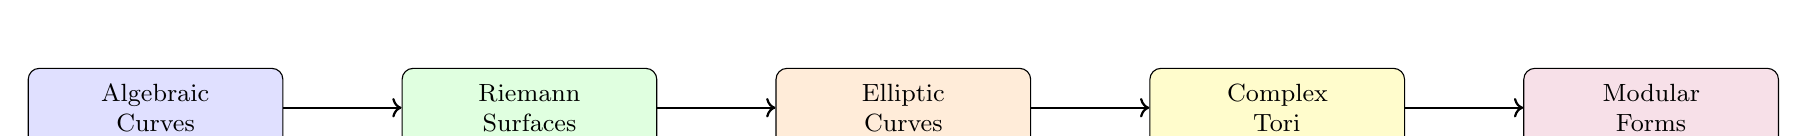
\begin{tikzpicture}[
			node distance=1.5cm,
			every node/.style={
				draw,
				rounded corners,
				align=center,
				text width=3cm,
				minimum height=1cm,
				font=\small
			},
			arrow/.style={->,thick}
			]
			
			\node[fill=blue!12] (curves) {Algebraic\\Curves};
			\node[fill=green!12,right=of curves] (rs) {Riemann\\Surfaces};
			\node[fill=orange!15,right=of rs] (ell) {Elliptic\\Curves};
			\node[fill=yellow!20,right=of ell] (torus) {Complex\\Tori};
			\node[fill=purple!12,right=of torus] (mod) {Modular\\Forms};
			
			\draw[arrow] (curves) -- (rs);
			\draw[arrow] (rs) -- (ell);
			\draw[arrow] (ell) -- (torus);
			\draw[arrow] (torus) -- (mod);
			
		\end{tikzpicture}
	}
\end{center}

Problem~16 leads toward analysis:

\begin{center}
	\resizebox{0.95\textwidth}{!}{%
		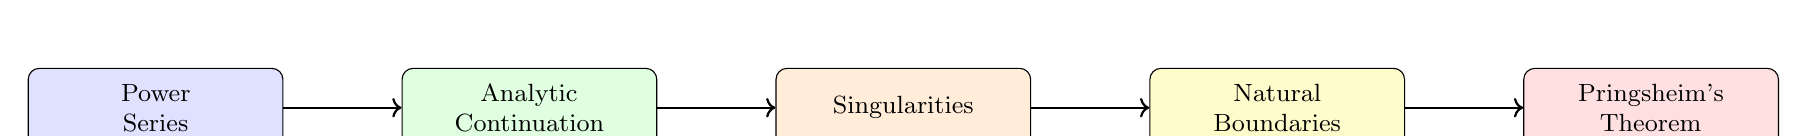
\begin{tikzpicture}[
			node distance=1.5cm,
			every node/.style={
				draw,
				rounded corners,
				align=center,
				text width=3cm,
				minimum height=1cm,
				font=\small
			},
			arrow/.style={->,thick}
			]
			
			\node[fill=blue!12] (ps) {Power\\Series};
			\node[fill=green!12,right=of ps] (ac) {Analytic\\Continuation};
			\node[fill=orange!15,right=of ac] (sing) {Singularities};
			\node[fill=yellow!20,right=of sing] (nb) {Natural\\Boundaries};
			\node[fill=red!12,right=of nb] (pr) {Pringsheim's\\Theorem};
			
			\draw[arrow] (ps) -- (ac);
			\draw[arrow] (ac) -- (sing);
			\draw[arrow] (sing) -- (nb);
			\draw[arrow] (nb) -- (pr);
			
		\end{tikzpicture}
	}
\end{center}

\bigskip

\subsection{Grand Synthesis}

\begin{center}
	\resizebox{0.95\textwidth}{!}{%
		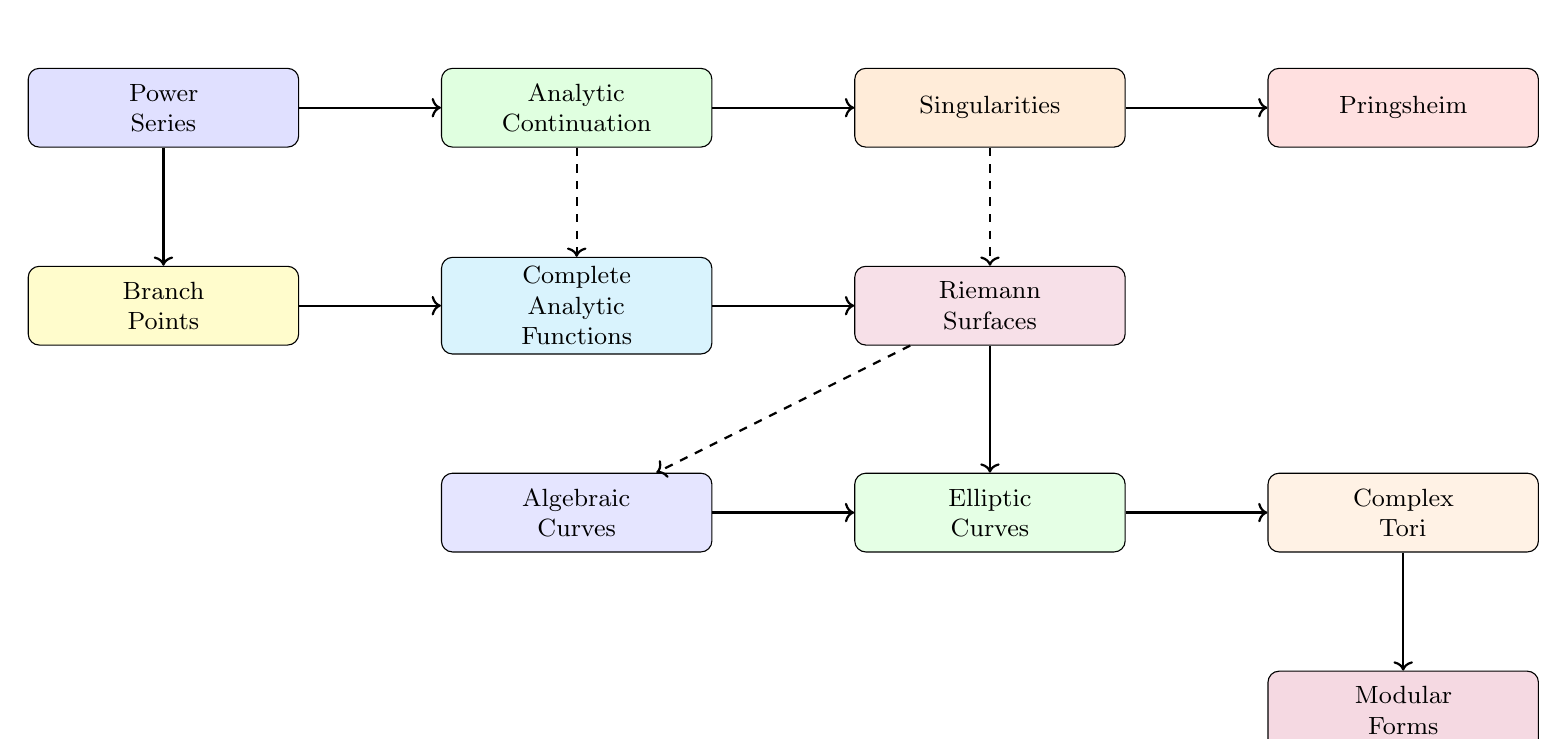
\begin{tikzpicture}[
			node distance=1.5cm and 1.8cm,
			every node/.style={
				draw,
				rounded corners,
				align=center,
				text width=3.2cm,
				minimum height=1cm,
				font=\small
			},
			arrow/.style={->,thick}
			]
			
			\node[fill=blue!12] (ps) {Power\\Series};
			\node[fill=green!12,right=of ps] (ac) {Analytic\\Continuation};
			\node[fill=orange!15,right=of ac] (sing) {Singularities};
			\node[fill=red!12,right=of sing] (pr) {Pringsheim};
			
			\node[fill=yellow!20,below=of ps] (bp) {Branch\\Points};
			\node[fill=cyan!15,right=of bp] (caf) {Complete\\Analytic\\Functions};
			\node[fill=purple!12,right=of caf] (rs) {Riemann\\Surfaces};
			
			\node[fill=blue!10,below=of caf] (curves) {Algebraic\\Curves};
			\node[fill=green!10,right=of curves] (ell) {Elliptic\\Curves};
			\node[fill=orange!10,right=of ell] (torus) {Complex\\Tori};
			
			\node[fill=purple!15,below=of torus] (mod) {Modular\\Forms};
			
			\draw[arrow] (ps) -- (ac);
			\draw[arrow] (ac) -- (sing);
			\draw[arrow] (sing) -- (pr);
			
			\draw[arrow] (ps) -- (bp);
			\draw[arrow] (bp) -- (caf);
			\draw[arrow] (caf) -- (rs);
			
			\draw[arrow] (rs) -- (ell);
			\draw[arrow] (curves) -- (ell);
			\draw[arrow] (ell) -- (torus);
			\draw[arrow] (torus) -- (mod);
			
			\draw[arrow,dashed] (ac) -- (caf);
			\draw[arrow,dashed] (sing) -- (rs);
			\draw[arrow,dashed] (rs) -- (curves);
			
		\end{tikzpicture}
	}
\end{center}

Thus Problems~15--16 represent the point where the theory splits into the two great directions of modern complex analysis:

\[
\boxed{
	\begin{gathered}
		\text{Geometry of Riemann Surfaces}\\[0.5ex]
		\text{and}\\[0.5ex]
		\text{Theory of Analytic Continuation}
	\end{gathered}
}
\]


\section{Detailed Examples for Problems 15--16}

The following examples illustrate the geometric and analytic ideas underlying Problems~15 and~16. They show how algebraic curves become Riemann surfaces and how singularities determine the behavior of power series.

\bigskip

\subsection{Example 1: The Surface \texorpdfstring{$w^2=z^3-z$}{w²=z³-z}}

Consider

\[
R
=
\{(z,w)\in\mathbb C^2:w^2=z^3-z\}.
\]

Since

\[
z^3-z
=
z(z-1)(z+1),
\]

the special values of \(z\) are

\[
z=-1,\qquad z=0,\qquad z=1.
\]

For example, if

\[
z=2,
\]

then

\[
w^2=2^3-2=6.
\]

Hence

\[
w=\pm\sqrt6.
\]

Thus over the point \(z=2\) there are two points on the surface:

\[
(2,\sqrt6),
\qquad
(2,-\sqrt6).
\]

Therefore the surface consists of two sheets lying above the \(z\)-plane.

\[
\boxed{
	\text{Two values of }w
	\Longleftrightarrow
	\text{Two sheets of the surface}.
}
\]

\bigskip

\subsection{Example 2: What Happens at a Branch Point?}

Take

\[
z=1.
\]

Then

\[
w^2=1^3-1=0,
\]

so

\[
w=0.
\]

The two branches

\[
+\sqrt{z^3-z},
\qquad
-\sqrt{z^3-z}
\]

coincide.

To study the local geometry, write

\[
z=1+\xi.
\]

Then

\[
z^3-z
=
(1+\xi)^3-(1+\xi)
=
2\xi+3\xi^2+\xi^3.
\]

Thus

\[
w^2
=
2\xi+O(\xi^2).
\]

Consequently

\[
w
=
\sqrt2\,\sqrt{\xi}
+O(\xi^{3/2}).
\]

Equivalently,

\[
w
\approx
\sqrt2\,\sqrt{z-1}.
\]

This is exactly the local model of a square-root branch point.

After one circuit around \(z=1\),

\[
\sqrt{z-1}
\longmapsto
-\sqrt{z-1}.
\]

Hence

\[
w
\longmapsto
-w.
\]

Therefore one loop exchanges the two sheets.

\bigskip

\subsection{Example 3: Local Coordinates Near a Ramification Point}

Consider the point

\[
(1,0)\in R.
\]

Near this point the coordinate \(z\) is not suitable because two sheets merge.

Instead use

\[
t=w.
\]

Define

\[
F(z,w)
=
w^2-z^3+z.
\]

Then

\[
F_z
=
-3z^2+1.
\]

At

\[
(1,0),
\]

we have

\[
F_z=-2\neq0.
\]

Therefore the implicit function theorem implies that

\[
z
\]

can be written as a holomorphic function of

\[
w.
\]

Expanding near \(w=0\),

\[
z
=
1+\frac12w^2+\cdots.
\]

Hence

\[
z
=
1+\frac12t^2+\cdots.
\]

The projection

\[
\pi(z,w)=z
\]

becomes

\[
t
\longmapsto
1+\frac12t^2+\cdots.
\]

Thus locally the covering looks like

\[
t\mapsto t^2,
\]

which is the standard ramified covering.

\bigskip

\subsection{Example 4: Removing Branch Points Produces a Covering}

Define

\[
R_0
=
R
\setminus
\{(-1,0),(0,0),(1,0)\}.
\]

Let

\[
U
=
\mathbb C
\setminus
\{-1,0,1\}.
\]

Choose a small simply connected domain

\[
V\subset U.
\]

Since

\[
z^3-z
\]

has no zeros on \(V\), there exists a holomorphic branch

\[
h(z)
=
\sqrt{z^3-z}.
\]

Then

\[
\pi^{-1}(V)
=
V_+
\sqcup
V_-,
\]

where

\[
V_+
=
\{(z,h(z)):z\in V\},
\]

and

\[
V_-
=
\{(z,-h(z)):z\in V\}.
\]

Each sheet projects biholomorphically onto \(V\).

Therefore

\[
\boxed{
	\pi:R_0
	\to
	\mathbb C\setminus\{-1,0,1\}
}
\]

is a two-sheeted covering map.

\bigskip

\subsection{Example 5: Monodromy Around Branch Points}

Choose the branch

\[
w=\sqrt{z^3-z}.
\]

A loop around any one of

\[
-1,\quad0,\quad1
\]

changes

\[
w
\mapsto
-w.
\]

Thus the action on sheets is

\[
(+)\leftrightarrow(-).
\]

Hence the monodromy group is

\[
\mathbb Z_2.
\]

The covering transformation is

\[
(z,w)
\longmapsto
(z,-w).
\]

This is the deck transformation exchanging the two sheets.

\bigskip

\subsection{Example 6: Computing the Genus}

Compactify the curve by adding the point at infinity.

The resulting map

\[
\overline R
\to
\widehat{\mathbb C}
\]

has degree \(2\) and four branch points:

\[
-1,\quad0,\quad1,\quad\infty.
\]

Apply the Riemann--Hurwitz formula:

\[
2g(\overline R)-2
=
2(2g(\widehat{\mathbb C})-2)
+
\sum(e_p-1).
\]

Since

\[
g(\widehat{\mathbb C})=0,
\]

and each branch point contributes \(1\),

\[
2g(\overline R)-2
=
2(-2)+4.
\]

Thus

\[
2g(\overline R)-2=0.
\]

Therefore

\[
g(\overline R)=1.
\]

Hence

\[
\boxed{
	w^2=z^3-z
}
\]

defines a torus.

It is therefore an elliptic curve.

\bigskip

\subsection{Example 7: Radius of Convergence from Singularities}

Consider

\[
f(z)
=
\frac1{1-z}.
\]

Its Taylor expansion at \(0\) is

\[
f(z)
=
\sum_{n=0}^{\infty}z^n.
\]

The nearest singularity is

\[
z=1.
\]

Since

\[
|1-0|=1,
\]

the radius of convergence is

\[
R=1.
\]

Now expand about

\[
w=\frac12.
\]

The nearest singularity is still \(1\), so

\[
\rho(1/2)
=
\left|1-\frac12\right|
=
\frac12.
\]

Thus

\[
\boxed{
	\rho(1/2)=\frac12.
}
\]

\bigskip

\subsection{Example 8: A Regular Boundary Point}

Consider

\[
f(z)
=
\frac1{1+z}.
\]

Its Taylor series at \(0\) is

\[
\sum_{n=0}^{\infty}
(-1)^n z^n.
\]

The radius of convergence is

\[
1,
\]

because the singularity occurs at

\[
z=-1.
\]

Take

\[
\zeta=1.
\]

Then

\[
\zeta/2=\frac12.
\]

The nearest singularity to \(1/2\) is \(-1\).

Hence

\[
\rho(1/2)
=
\left|
\frac12-(-1)
\right|
=
\frac32.
\]

Since

\[
\frac32>\frac12,
\]

the point \(1\) is regular.

Thus

\[
\boxed{
	\rho(\zeta/2)>\frac12
	\Longrightarrow
	\zeta
	\text{ is regular}.
}
\]

\bigskip

\subsection{Example 9: Pringsheim's Theorem}

Consider

\[
f(z)
=
\sum_{n=0}^{\infty}z^n
=
\frac1{1-z}.
\]

All coefficients satisfy

\[
a_n=1\ge0.
\]

The radius of convergence is

\[
R=1.
\]

Pringsheim's theorem states that

\[
z=R
\]

must be singular.

Indeed,

\[
z=1
\]

is a pole.

Thus

\[
\boxed{
	a_n\ge0
	\Longrightarrow
	z=R
	\text{ is singular}.
}
\]

\bigskip

\subsection{Example 10: Another Positive-Coefficient Example}

Consider

\[
f(z)
=
\sum_{n=0}^{\infty}
2^n z^n.
\]

Summing the geometric series,

\[
f(z)
=
\frac1{1-2z}.
\]

The radius of convergence is

\[
R=\frac12.
\]

The singularity occurs exactly at

\[
z=\frac12.
\]

Again the positive real boundary point is singular.

This is another illustration of Pringsheim's theorem.

\bigskip

\subsection{Example 11: Catalan Numbers}

Let

\[
C_n
=
\frac1{n+1}
\binom{2n}{n}.
\]

The generating function is

\[
F(z)
=
\sum_{n=0}^{\infty}
C_n z^n
=
\frac{1-\sqrt{1-4z}}{2z}.
\]

The singularity occurs when

\[
1-4z=0.
\]

Hence

\[
z=\frac14.
\]

The radius of convergence is

\[
R=\frac14.
\]

The singularity is not a pole but a branch point.

Thus Pringsheim's theorem applies even to non-pole singularities.

\bigskip

\subsection{Example 12: Why Positivity Matters}

Consider

\[
f(z)
=
\sum_{n=0}^{\infty}
(-1)^n z^n
=
\frac1{1+z}.
\]

The radius of convergence is

\[
1.
\]

However

\[
z=1
\]

is perfectly regular:

\[
f(1)=\frac12.
\]

The singularity occurs at

\[
z=-1.
\]

Thus without positivity the conclusion of Pringsheim's theorem fails.

Therefore the condition

\[
a_n\ge0
\]

is essential.

\bigskip

\subsection{Final Interpretation}

Problem~15 teaches:

\[
\boxed{
	\text{Multivalued algebraic functions become single-valued on Riemann surfaces.}
}
\]

Problem~16 teaches:

\[
\boxed{
	\text{The radius of convergence is controlled by singularities,}
}
\]

and

\[
\boxed{
	\text{Positive coefficients force a singularity at the positive real boundary point.}
}
\]

Together these problems connect the geometry of algebraic curves with the analytic theory of power series and singularities.

\section{Colored Diagrams, Tables, and Visual Schemes for Problems 15--16}

\subsection{Geometric Roadmap}

\begin{center}
	\resizebox{0.92\textwidth}{!}{
		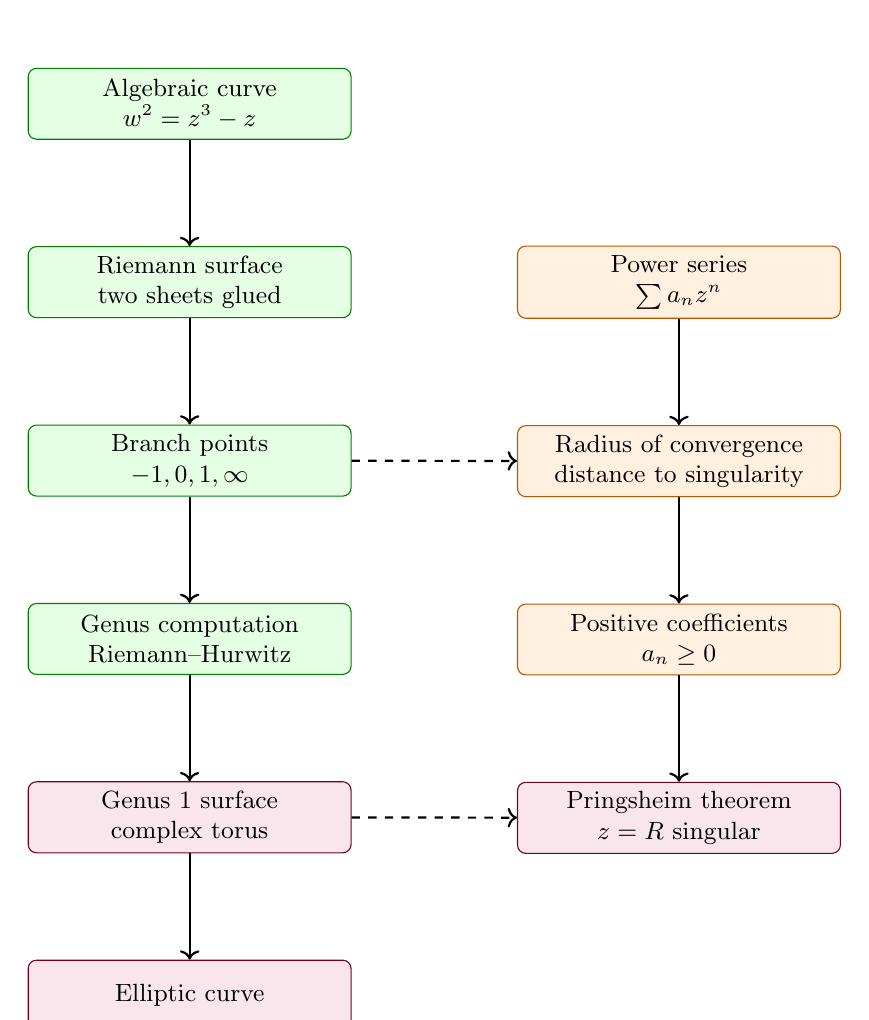
\begin{tikzpicture}[
			node distance=1.35cm,
			box/.style={
				draw,
				rounded corners=3pt,
				minimum width=4.1cm,
				minimum height=0.9cm,
				align=center,
				font=\small,
				fill=blue!8
			},
			geom/.style={box,fill=green!10,draw=green!50!black},
			anal/.style={box,fill=orange!12,draw=orange!70!black},
			final/.style={box,fill=purple!10,draw=purple!60!black},
			arrow/.style={->,thick}
			]
			
			\node[geom] (alg) {Algebraic curve\\ \(w^2=z^3-z\)};
			\node[geom,below=of alg] (rs) {Riemann surface\\ two sheets glued};
			\node[geom,below=of rs] (branch) {Branch points\\ \(-1,0,1,\infty\)};
			\node[geom,below=of branch] (genus) {Genus computation\\ Riemann--Hurwitz};
			\node[final,below=of genus] (torus) {Genus \(1\) surface\\ complex torus};
			\node[final,below=of torus] (ell) {Elliptic curve};
			
			\node[anal,right=2.1cm of rs] (series) {Power series\\ \(\sum a_nz^n\)};
			\node[anal,below=of series] (radius) {Radius of convergence\\ distance to singularity};
			\node[anal,below=of radius] (pos) {Positive coefficients\\ \(a_n\ge0\)};
			\node[final,below=of pos] (pring) {Pringsheim theorem\\ \(z=R\) singular};
			
			\draw[arrow] (alg)--(rs);
			\draw[arrow] (rs)--(branch);
			\draw[arrow] (branch)--(genus);
			\draw[arrow] (genus)--(torus);
			\draw[arrow] (torus)--(ell);
			
			\draw[arrow] (series)--(radius);
			\draw[arrow] (radius)--(pos);
			\draw[arrow] (pos)--(pring);
			
			\draw[arrow,dashed] (branch)--(radius);
			\draw[arrow,dashed] (torus)--(pring);
			
		\end{tikzpicture}
	}
\end{center}

\subsection{Branch Points of \texorpdfstring{$w^2=z^3-z$}{w2=z3-z}}

Since

\[
z^3-z=z(z-1)(z+1),
\]

the finite branch points are

\[
-1,\qquad 0,\qquad 1.
\]

The compactified curve also has a branch point at infinity.

\begin{center}
	\resizebox{0.85\textwidth}{!}{
		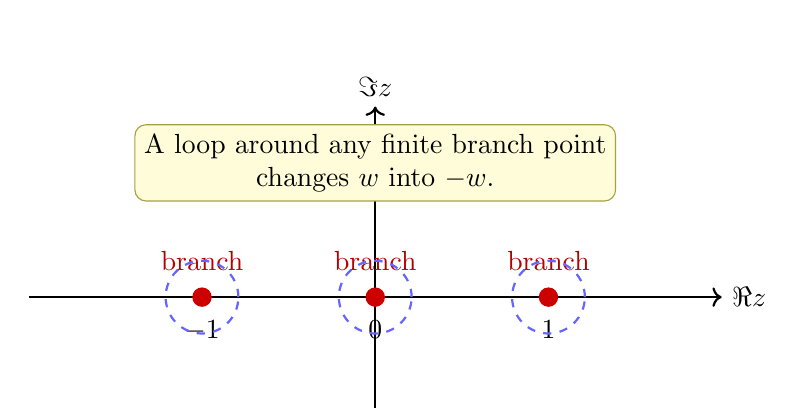
\begin{tikzpicture}[scale=1.1]
			
			\draw[->,thick] (-4,0)--(4,0) node[right] {\(\Re z\)};
			\draw[->,thick] (0,-1.4)--(0,2.2) node[above] {\(\Im z\)};
			
			\foreach \x/\lab in {-2/-1,0/0,2/1}
			{
				\filldraw[red!80!black] (\x,0) circle (3pt);
				\node[below=5pt] at (\x,0) {\(\lab\)};
				\node[above=6pt,red!70!black] at (\x,0) {branch};
			}
			
			\draw[blue!60,thick,dashed] (-2,0) circle (0.42);
			\draw[blue!60,thick,dashed] (0,0) circle (0.42);
			\draw[blue!60,thick,dashed] (2,0) circle (0.42);
			
			\node[align=center,fill=yellow!15,draw=yellow!60!black,rounded corners] at (0,1.55)
			{A loop around any finite branch point\\changes \(w\) into \(-w\).};
			
		\end{tikzpicture}
	}
\end{center}

\subsection{Two-Sheeted Covering Picture}

Away from the branch points, the projection

\[
\pi:R_0\to \mathbb C\setminus\{-1,0,1\}
\]

is a two-sheeted covering.

\begin{center}
	\resizebox{0.9\textwidth}{!}{
		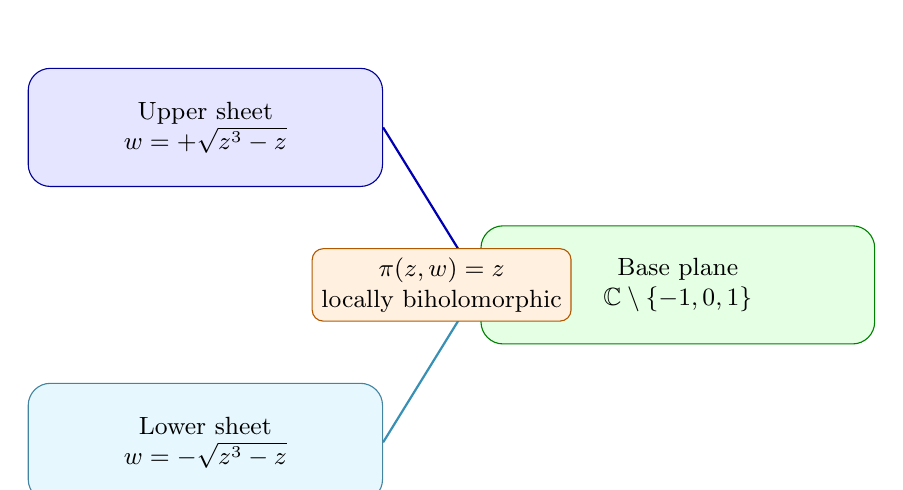
\begin{tikzpicture}[
			sheet/.style={
				draw,
				rounded corners=8pt,
				minimum width=4.5cm,
				minimum height=1.5cm,
				align=center,
				font=\small
			},
			arrow/.style={->,thick}
			]
			
			\node[sheet,fill=blue!10,draw=blue!60!black] (upper) at (-3,2)
			{Upper sheet\\ \(w=+\sqrt{z^3-z}\)};
			
			\node[sheet,fill=cyan!10,draw=cyan!60!black] (lower) at (-3,-2)
			{Lower sheet\\ \(w=-\sqrt{z^3-z}\)};
			
			\node[sheet,fill=green!10,draw=green!50!black,minimum width=5cm] (base) at (3,0)
			{Base plane\\ \(\mathbb C\setminus\{-1,0,1\}\)};
			
			\draw[arrow,blue!70!black] (upper.east)--(base.west);
			\draw[arrow,cyan!70!black] (lower.east)--(base.west);
			
			\node[fill=orange!12,draw=orange!70!black,rounded corners,align=center,font=\small] at (0,0)
			{\(\pi(z,w)=z\)\\ locally biholomorphic};
			
		\end{tikzpicture}
	}
\end{center}

\subsection{Local Ramification Model}

Near a branch point \(z_0\), the curve has the local form

\[
w^2\sim z-z_0.
\]

Using \(t=w\) as a local coordinate,

\[
z=z_0+ct^2+\cdots.
\]

Thus locally the projection behaves like

\[
t\mapsto t^2.
\]

\begin{center}
	\resizebox{0.82\textwidth}{!}{
		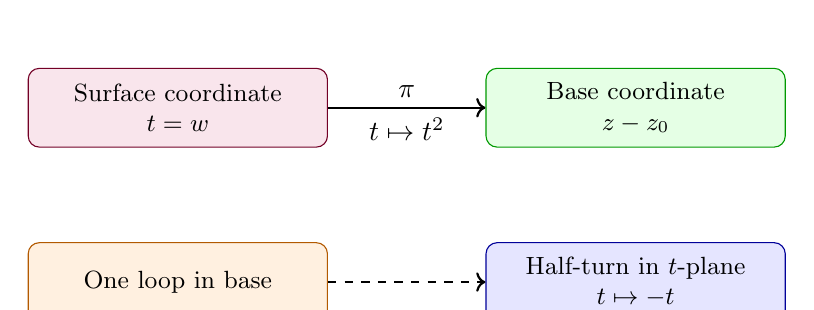
\begin{tikzpicture}[
			node distance=2cm,
			box/.style={
				draw,
				rounded corners,
				align=center,
				font=\small,
				minimum width=3.8cm,
				minimum height=1cm
			},
			arrow/.style={->,thick}
			]
			
			\node[box,fill=purple!10,draw=purple!60!black] (surface)
			{Surface coordinate\\ \(t=w\)};
			
			\node[box,fill=green!10,draw=green!60!black,right=of surface] (base)
			{Base coordinate\\ \(z-z_0\)};
			
			\draw[arrow] (surface)--node[above] {\(\pi\)} node[below] {\(t\mapsto t^2\)} (base);
			
			\node[box,fill=orange!12,draw=orange!70!black,below=1.2cm of surface] (loop1)
			{One loop in base};
			
			\node[box,fill=blue!10,draw=blue!60!black,below=1.2cm of base] (loop2)
			{Half-turn in \(t\)-plane\\ \(t\mapsto -t\)};
			
			\draw[arrow,dashed] (loop1)--(loop2);
			
		\end{tikzpicture}
	}
\end{center}

\subsection{Riemann--Hurwitz Genus Calculation}

For the compactified curve

\[
\overline R:\quad w^2=z^3-z,
\]

the map

\[
\overline R\to\widehat{\mathbb C}
\]

has degree \(2\) and four branch points:

\[
-1,\quad0,\quad1,\quad\infty.
\]

Therefore

\[
2g(\overline R)-2
=
2(2g(\widehat{\mathbb C})-2)+4.
\]

Since

\[
g(\widehat{\mathbb C})=0,
\]

we get

\[
2g(\overline R)-2
=
2(-2)+4=0.
\]

Hence

\[
g(\overline R)=1.
\]

\begin{center}
	\[
	\begin{array}{c|c|c|c}
		\rowcolor{blue!12}
		\textbf{Object} &
		\textbf{Degree} &
		\textbf{Branch points} &
		\textbf{Genus}
		\\
		\hline
		\widehat{\mathbb C} &
		1 &
		\text{none} &
		0
		\\
		\hline
		w^2=z &
		2 &
		0,\infty &
		0
		\\
		\hline
		\rowcolor{green!10}
		w^2=z^3-z &
		2 &
		-1,0,1,\infty &
		1
		\\
		\hline
		w^2=z^5-z &
		2 &
		\text{six branch points} &
		2
	\end{array}
	\]
\end{center}

\subsection{Genus Ladder}

\begin{center}
	\resizebox{0.92\textwidth}{!}{
		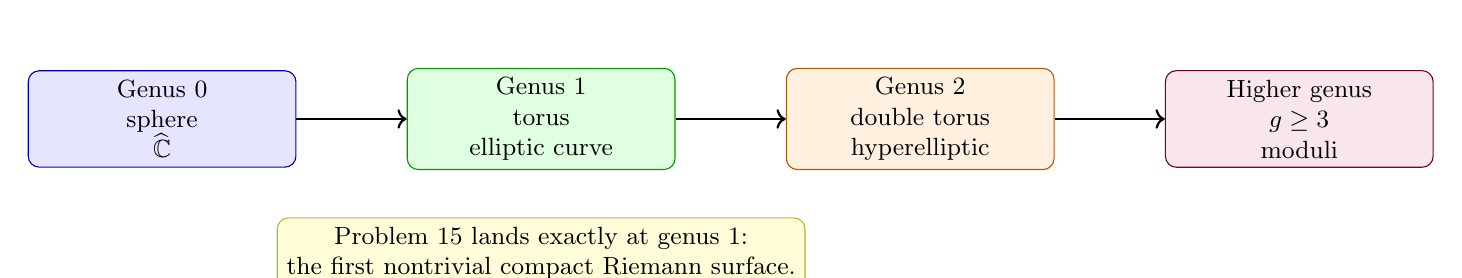
\begin{tikzpicture}[
			node distance=1.4cm,
			box/.style={
				draw,
				rounded corners,
				minimum width=3.4cm,
				minimum height=1cm,
				align=center,
				font=\small
			},
			arrow/.style={->,thick}
			]
			
			\node[box,fill=blue!10,draw=blue!70!black] (g0)
			{Genus \(0\)\\ sphere\\ \(\widehat{\mathbb C}\)};
			
			\node[box,fill=green!12,draw=green!60!black,right=of g0] (g1)
			{Genus \(1\)\\ torus\\ elliptic curve};
			
			\node[box,fill=orange!12,draw=orange!70!black,right=of g1] (g2)
			{Genus \(2\)\\ double torus\\ hyperelliptic};
			
			\node[box,fill=purple!10,draw=purple!60!black,right=of g2] (gn)
			{Higher genus\\ \(g\ge3\)\\ moduli};
			
			\draw[arrow] (g0)--(g1);
			\draw[arrow] (g1)--(g2);
			\draw[arrow] (g2)--(gn);
			
			\node[below=0.6cm of g1,align=center,font=\small,fill=yellow!15,draw=yellow!70!black,rounded corners]
			{Problem 15 lands exactly at genus \(1\):\\ the first nontrivial compact Riemann surface.};
			
		\end{tikzpicture}
	}
\end{center}

\subsection{Radius of Convergence Geometry}

For a power series centered at \(0\), the radius of convergence is the distance to the nearest singularity.

For a Taylor expansion centered at \(w\), the radius is denoted

\[
\rho(w).
\]

In Problem~16, the key point is

\[
w=\frac{\zeta}{2},
\qquad
|\zeta|=1.
\]

Then

\[
\left|\zeta-\frac{\zeta}{2}\right|=\frac12.
\]

\begin{center}
	\resizebox{0.72\textwidth}{!}{
		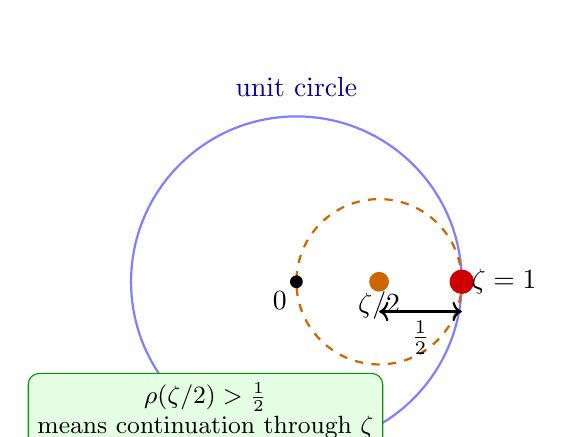
\begin{tikzpicture}[scale=2.1]
			
			\draw[thick,blue!50] (0,0) circle (1);
			\node[blue!60!black] at (0,1.18) {unit circle};
			
			\draw[dashed,orange!80!black,thick] (0.5,0) circle (0.5);
			
			\filldraw[black] (0,0) circle (1pt);
			\node[below left] at (0,0) {\(0\)};
			
			\filldraw[red!80!black] (1,0) circle (2pt);
			\node[right] at (1,0) {\(\zeta=1\)};
			
			\filldraw[orange!80!black] (0.5,0) circle (1.6pt);
			\node[below] at (0.5,0) {\(\zeta/2\)};
			
			\draw[<->,thick] (0.5,-0.18)--(1,-0.18);
			\node[below] at (0.75,-0.18) {\(\frac12\)};
			
			\node[align=center,fill=green!10,draw=green!60!black,rounded corners,font=\small] at (-0.55,-0.78)
			{\(\rho(\zeta/2)>\frac12\)\\ means continuation through \(\zeta\)};
			
		\end{tikzpicture}
	}
\end{center}

\subsection{Regular Versus Singular Boundary Point}

\[
\begin{array}{c|c|c}
	\rowcolor{purple!12}
	\textbf{Condition} &
	\textbf{Geometric meaning} &
	\textbf{Boundary behavior}
	\\
	\hline
	\rho(\zeta/2)>\frac12
	&
	\text{Taylor disc crosses the unit circle}
	&
	\text{\(\zeta\) is regular}
	\\
	\hline
	\rho(\zeta/2)=\frac12
	&
	\text{Taylor disc touches a singular obstruction}
	&
	\text{\(\zeta\) is singular}
	\\
	\hline
	\rho(\zeta/2)<\frac12
	&
	\text{Singularity occurs before reaching \(\zeta\)}
	&
	\text{\(\zeta\) cannot be reached from that center}
\end{array}
\]

\subsection{Pringsheim's Theorem Flowchart}

\begin{center}
	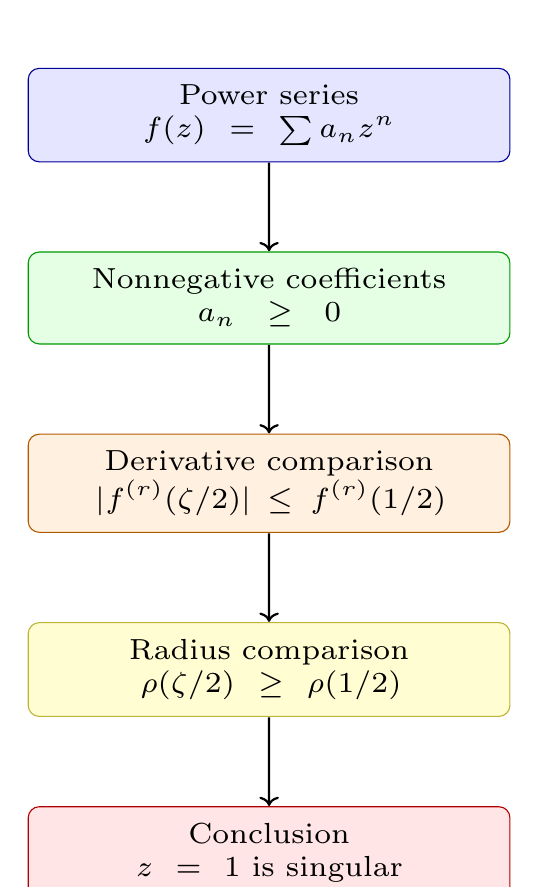
\begin{tikzpicture}[
		scale= 1.499,
		transform shape,
		node distance=0.75cm,
		box/.style={
			draw,
			rounded corners,
			align=center,
			font=\scriptsize,
			text width=3.8cm,
			minimum height=0.75cm,
			inner sep=4pt
		},
		arrow/.style={->,thick}
		]
		
		\node[box,fill=blue!10,draw=blue!60!black] (series)
		{Power series\\ \(f(z)=\sum a_nz^n\)};
		
		\node[box,fill=green!10,draw=green!60!black,below=of series] (pos)
		{Nonnegative coefficients\\ \(a_n\ge0\)};
		
		\node[box,fill=orange!12,draw=orange!70!black,below=of pos] (ineq)
		{Derivative comparison\\
			\(|f^{(r)}(\zeta/2)|\le f^{(r)}(1/2)\)};
		
		\node[box,fill=yellow!18,draw=yellow!70!black,below=of ineq] (rho)
		{Radius comparison\\
			\(\rho(\zeta/2)\ge\rho(1/2)\)};
		
		\node[box,fill=red!10,draw=red!70!black,below=of rho] (sing)
		{Conclusion\\ \(z=1\) is singular};
		
		\draw[arrow] (series) -- (pos);
		\draw[arrow] (pos) -- (ineq);
		\draw[arrow] (ineq) -- (rho);
		\draw[arrow] (rho) -- (sing);
		
	\end{tikzpicture}
\end{center}

\subsection{Positive and Non-Positive Coefficient Comparison}

\[
\begin{array}{c|c|c|c}
	\rowcolor{blue!12}
	\textbf{Series} &
	\textbf{Coefficients} &
	\textbf{Radius} &
	\textbf{Singularity on boundary}
	\\
	\hline
	\displaystyle \sum_{n=0}^{\infty} z^n
	&
	a_n=1\ge0
	&
	1
	&
	z=1
	\\
	\hline
	\displaystyle \sum_{n=0}^{\infty} 2^n z^n
	&
	a_n=2^n\ge0
	&
	\frac12
	&
	z=\frac12
	\\
	\hline
	\displaystyle \sum_{n=0}^{\infty} C_n z^n
	&
	C_n\ge0
	&
	\frac14
	&
	z=\frac14
	\\
	\hline
	\rowcolor{red!8}
	\displaystyle \sum_{n=0}^{\infty}(-1)^n z^n
	&
	\text{not nonnegative}
	&
	1
	&
	z=-1
\end{array}
\]

\subsection{Problem 15 Versus Problem 16}

\[
\begin{array}{c|c|c}
	\rowcolor{green!12}
	&
	\textbf{Problem 15}
	&
	\textbf{Problem 16}
	\\
	\hline
	\textbf{Main object}
	&
	\displaystyle w^2=z^3-z
	&
	\displaystyle \sum a_nz^n
	\\
	\hline
	\textbf{Main viewpoint}
	&
	\text{Geometry}
	&
	\text{Analysis}
	\\
	\hline
	\textbf{Key obstruction}
	&
	\text{Branch points}
	&
	\text{Singular boundary points}
	\\
	\hline
	\textbf{Main construction}
	&
	\text{Riemann surface}
	&
	\text{Taylor discs}
	\\
	\hline
	\textbf{Main theorem}
	&
	\text{Riemann--Hurwitz}
	&
	\text{Pringsheim theorem}
	\\
	\hline
	\textbf{Outcome}
	&
	\text{Elliptic curve}
	&
	\text{Positive real singularity}
	\\
	\hline
	\textbf{Future direction}
	&
	\text{Algebraic geometry}
	&
	\text{Analytic combinatorics}
\end{array}
\]

\subsection{Final Concept Diagram}

\begin{center}
	\resizebox{0.95\textwidth}{!}{
		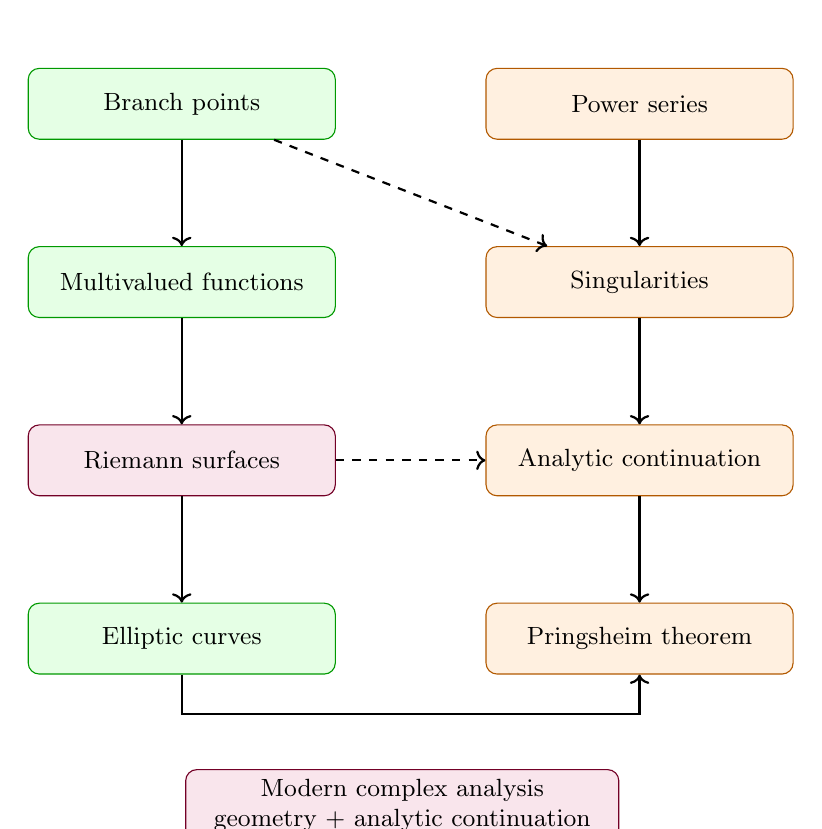
\begin{tikzpicture}[
			node distance=1.35cm and 1.9cm,
			box/.style={
				draw,
				rounded corners,
				align=center,
				font=\small,
				minimum width=3.9cm,
				minimum height=0.9cm
			},
			geom/.style={box,fill=green!10,draw=green!60!black},
			anal/.style={box,fill=orange!12,draw=orange!70!black},
			core/.style={box,fill=purple!10,draw=purple!60!black},
			arrow/.style={->,thick}
			]
			
			\node[geom] (branch) {Branch points};
			\node[geom,below=of branch] (multi) {Multivalued functions};
			\node[core,below=of multi] (rs) {Riemann surfaces};
			\node[geom,below=of rs] (ell) {Elliptic curves};
			
			\node[anal,right=of branch] (series) {Power series};
			\node[anal,below=of series] (sing) {Singularities};
			\node[anal,below=of sing] (cont) {Analytic continuation};
			\node[anal,below=of cont] (pring) {Pringsheim theorem};
			
			\draw[arrow] (branch)--(multi);
			\draw[arrow] (multi)--(rs);
			\draw[arrow] (rs)--(ell);
			
			\draw[arrow] (series)--(sing);
			\draw[arrow] (sing)--(cont);
			\draw[arrow] (cont)--(pring);
			
			\draw[arrow,dashed] (branch)--(sing);
			\draw[arrow,dashed] (rs)--(cont);
			
			\node[core,below=1.2cm of ell,xshift=2.8cm,minimum width=5.5cm]
			{Modern complex analysis\\ geometry \(+\) analytic continuation};
			
			\draw[arrow] (ell.south)--++(0,-0.5)-| (pring.south);
			
		\end{tikzpicture}
	}
\end{center}

\section{Examples Illustrating Pringsheim's Theorem}

Recall Pringsheim's theorem.

\begin{theorem}[Pringsheim]
	Let
	\[
	f(z)=\sum_{n=0}^{\infty} a_n z^n
	\]
	be a power series with nonnegative coefficients
	\[
	a_n\ge 0.
	\]
	Suppose the radius of convergence is \(R<\infty\). Then the point
	\[
	z=R
	\]
	is a singular point of \(f\).
\end{theorem}

The theorem states that for power series with nonnegative coefficients, the first singularity necessarily lies on the positive real axis.

\bigskip

\subsection{Example 1: The Geometric Series}

Consider
\[
f(z)=1+z+z^2+z^3+\cdots.
\]

All coefficients satisfy

\[
a_n=1\ge0.
\]

\subsubsection*{Step 1: Radius of Convergence}

Using the Cauchy--Hadamard formula,

\[
R=
\frac{1}
{\limsup\limits_{n\to\infty}\sqrt[n]{1}}
=
1.
\]

\subsubsection*{Step 2: Sum of the Series}

For \(|z|<1\),

\[
f(z)=\frac{1}{1-z}.
\]

\subsubsection*{Step 3: Singularities}

The denominator vanishes when

\[
1-z=0,
\]

hence

\[
z=1.
\]

Therefore \(z=1\) is a pole.

\subsubsection*{Conclusion}

Since

\[
R=1,
\]

the boundary point

\[
z=R=1
\]

is singular, exactly as predicted by Pringsheim's theorem.

\begin{center}
	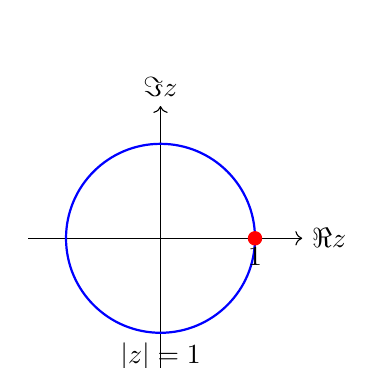
\begin{tikzpicture}[scale=1.2]
		\draw[->] (-1.4,0)--(1.5,0) node[right] {\(\Re z\)};
		\draw[->] (0,-1.4)--(0,1.4) node[above] {\(\Im z\)};
		\draw[blue,thick] (0,0) circle (1);
		\filldraw[red] (1,0) circle (2pt);
		\node[below] at (1,0) {\(1\)};
		\node at (0,-1.25) {\(|z|=1\)};
	\end{tikzpicture}
\end{center}

\bigskip

\subsection{Example 2: The Logarithm}

Consider

\[
f(z)=
\sum_{n=1}^{\infty}
\frac{z^n}{n}.
\]

All coefficients satisfy

\[
a_n=\frac1n>0.
\]

\subsubsection*{Step 1: Radius of Convergence}

Since

\[
\lim_{n\to\infty}\sqrt[n]{\frac1n}=1,
\]

we obtain

\[
R=1.
\]

\subsubsection*{Step 2: Closed Form}

Inside the unit disk,

\[
f(z)= -\log(1-z).
\]

\subsubsection*{Step 3: Singularity}

The logarithm becomes singular at

\[
1-z=0,
\]

that is,

\[
z=1.
\]

This is a branch point.

\subsubsection*{Conclusion}

Again,

\[
R=1
\]

and

\[
z=R
\]

is singular.

\begin{center}
	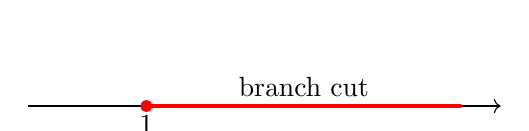
\begin{tikzpicture}
		\draw[->] (-0.5,0)--(5.5,0);
		\filldraw[red] (1,0) circle (2pt);
		\node[below] at (1,0) {\(1\)};
		\draw[very thick,red] (1,0)--(5,0);
		\node[above] at (3,0) {branch cut};
	\end{tikzpicture}
\end{center}

\bigskip

\subsection{Example 3: An Entire Function}

Consider

\[
f(z)=
\sum_{n=0}^{\infty}
\frac{z^n}{(n!)^2}.
\]

All coefficients are positive.

\subsubsection*{Radius of Convergence}

Since

\[
\sqrt[n]{\frac1{(n!)^2}}
\longrightarrow 0,
\]

we obtain

\[
R=\infty.
\]

\subsubsection*{Interpretation}

The function converges everywhere.

Indeed,

\[
f(z)=I_0(2\sqrt z),
\]

where \(I_0\) is the modified Bessel function.

\subsubsection*{Conclusion}

The function is entire.

Since \(R=\infty\), Pringsheim's theorem does not apply because there is no finite boundary circle.

\bigskip

\subsection{Example 4: Catalan Numbers}

Consider the generating function

\[
C(z)=
\sum_{n=0}^{\infty}
C_n z^n,
\]

where

\[
C_n=
\frac1{n+1}
\binom{2n}{n}.
\]

\subsubsection*{Step 1: Radius of Convergence}

Using Stirling's formula,

\[
C_n
\sim
\frac{4^n}
{n^{3/2}\sqrt{\pi}}.
\]

Therefore

\[
R=\frac14.
\]

\subsubsection*{Step 2: Closed Formula}

One has

\[
C(z)
=
\frac{1-\sqrt{1-4z}}
{2z}.
\]

\subsubsection*{Step 3: Singular Point}

The square root becomes singular when

\[
1-4z=0.
\]

Hence

\[
z=\frac14.
\]

\subsubsection*{Conclusion}

The singularity occurs exactly at

\[
z=R=\frac14.
\]

\begin{center}
	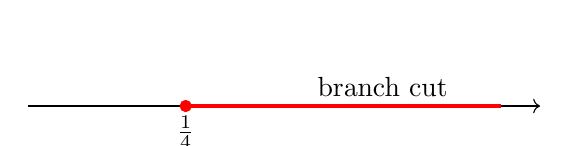
\begin{tikzpicture}
		\draw[->] (-0.5,0)--(6,0);
		\filldraw[red] (1.5,0) circle (2pt);
		\node[below] at (1.5,0) {\(\frac14\)};
		\draw[very thick,red] (1.5,0)--(5.5,0);
		\node[above] at (4,0) {branch cut};
	\end{tikzpicture}
\end{center}

\bigskip

\subsection{Example 5: Partition Numbers}

Let

\[
P(z)=
\sum_{n=0}^{\infty}
p(n)z^n,
\]

where \(p(n)\) denotes the number of integer partitions of \(n\).

Euler discovered the product formula

\[
P(z)
=
\prod_{m=1}^{\infty}
\frac1{1-z^m}.
\]

All coefficients satisfy

\[
p(n)\ge0.
\]

\subsubsection*{Radius of Convergence}

One finds

\[
R=1.
\]

\subsubsection*{Singularity}

At

\[
z=1,
\]

every factor

\[
\frac1{1-z^m}
\]

becomes singular.

Therefore the product diverges.

\subsubsection*{Conclusion}

The point

\[
z=1
\]

is a singularity, exactly as predicted by Pringsheim's theorem.

\bigskip

\subsection{Comparison Table}

\begin{center}
	\renewcommand{\arraystretch}{1.4}
	\begin{tabular}{|c|c|c|c|}
		\hline
		Function & Radius \(R\) & Singular at \(R\)? & Type \\
		\hline
		\(\dfrac1{1-z}\) & \(1\) & Yes & Pole \\
		\hline
		\(-\log(1-z)\) & \(1\) & Yes & Branch point \\
		\hline
		\(\sum \dfrac{z^n}{(n!)^2}\) & \(\infty\) & Not applicable & Entire \\
		\hline
		Catalan generating function & \(\frac14\) & Yes & Square-root branch \\
		\hline
		Partition generating function & \(1\) & Yes & Infinite-product singularity \\
		\hline
	\end{tabular}
\end{center}

\bigskip

\subsection{Summary}

Pringsheim's theorem can be summarized as

\[
\boxed{
	\text{Nonnegative coefficients}
	\Longrightarrow
	\text{a singularity occurs at the positive radius } R.
}
\]

This result is one of the central tools of analytic combinatorics and explains why the asymptotic behavior of counting sequences such as

\[
C_n,\qquad p(n),\qquad
\text{Motzkin numbers},\qquad
\text{Fibonacci numbers},
\]

is governed by the first singularity of their generating function on the positive real axis.

\section{Pringsheim's Theorem and Modular Forms}

Pringsheim's theorem is usually introduced in complex analysis and analytic combinatorics, but one of its deepest applications occurs in the theory of modular forms.

The bridge between the two subjects is provided by generating functions whose coefficients count arithmetic objects.

\bigskip

\subsection{The Partition Function}

Let

\[
p(n)
\]

denote the number of partitions of \(n\).

For example,

\[
4=4=3+1=2+2=2+1+1=1+1+1+1,
\]

so

\[
p(4)=5.
\]

Euler proved that the generating function is

\[
P(q)
=
\sum_{n=0}^{\infty}
p(n)q^n
=
\prod_{m=1}^{\infty}
\frac{1}{1-q^m}.
\]

The coefficients satisfy

\[
p(n)\ge0.
\]

Therefore Pringsheim's theorem applies.

\bigskip

Since the radius of convergence is

\[
R=1,
\]

the point

\[
q=1
\]

must be singular.

Indeed,

\[
\prod_{m=1}^{\infty}
\frac{1}{1-q^m}
\]

blows up as \(q\to1^{-}\).

Thus the dominant singularity occurs exactly at the positive real boundary point.

\bigskip

\subsection{The Dedekind Eta Function}

The infinite product above is closely related to the Dedekind eta function

\[
\eta(\tau)
=
q^{1/24}
\prod_{n=1}^{\infty}
(1-q^n),
\]

where

\[
q=e^{2\pi i\tau},
\qquad
\Im(\tau)>0.
\]

Hence

\[
P(q)
=
\frac{q^{-1/24}}{\eta(\tau)}.
\]

The partition generating function is therefore essentially the reciprocal of a modular form.

\bigskip

This remarkable observation connects

\[
\text{Combinatorics}
\quad\longleftrightarrow\quad
\text{Modular Forms}.
\]

\bigskip

\subsection{Why the Singularity at \(q=1\) Matters}

Pringsheim's theorem tells us where the dominant singularity is located:

\[
q=1.
\]

Near this point,

\[
P(q)
=
\prod_{m=1}^{\infty}
\frac1{1-q^m}
\]

grows extremely rapidly.

The asymptotic growth of the coefficients

\[
p(n)
\]

is controlled by the behavior of the generating function near this singularity.

This principle is fundamental in analytic combinatorics:

\[
\boxed{
	\text{Coefficient growth}
	\Longleftrightarrow
	\text{Boundary singularities}
}
\]

\bigskip

\subsection{Hardy--Ramanujan Asymptotics}

Using the modular properties of the eta function, Hardy and Ramanujan proved

\[
p(n)
\sim
\frac{1}
{4n\sqrt3}
\exp\!\left(
\pi
\sqrt{\frac{2n}{3}}
\right).
\]

This is one of the most celebrated results in analytic number theory.

The argument begins with the singularity at

\[
q=1,
\]

whose existence is guaranteed by Pringsheim's theorem.

\bigskip

Thus the logical chain is

\[
\text{Positive coefficients}
\Longrightarrow
q=1\text{ singular}
\Longrightarrow
\text{modular analysis}
\Longrightarrow
\text{asymptotics of }p(n).
\]

\bigskip

\subsection{Modular Forms Beyond Partitions}

Many modular forms possess Fourier expansions

\[
f(\tau)
=
\sum_{n=0}^{\infty}
a_n q^n,
\qquad
q=e^{2\pi i\tau}.
\]

Examples include

\[
E_4(\tau),
\qquad
E_6(\tau),
\qquad
\Delta(\tau),
\qquad
\eta(\tau).
\]

Their coefficients encode deep arithmetic information:

\begin{center}
	\renewcommand{\arraystretch}{1.3}
	\begin{tabular}{|c|c|}
		\hline
		Modular Form & Information Encoded \\
		\hline
		\(\eta(\tau)\) & Partitions \\
		\hline
		\(E_4(\tau)\) & Divisor sums \\
		\hline
		\(E_6(\tau)\) & Divisor sums \\
		\hline
		\(\Delta(\tau)\) & Ramanujan \(\tau(n)\) \\
		\hline
		Theta functions & Representations by quadratic forms \\
		\hline
	\end{tabular}
\end{center}

Although coefficients of modular forms are not always nonnegative, whenever a generating function has nonnegative coefficients, Pringsheim's theorem identifies the dominant boundary singularity and often provides the first step toward asymptotic analysis.

\bigskip

\subsection{Conceptual Diagram}

\begin{center}
	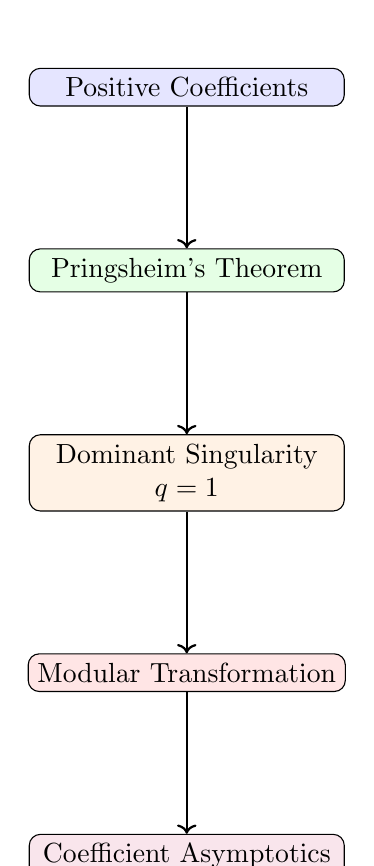
\begin{tikzpicture}[
		node distance=1.8cm,
		every node/.style={
			draw,
			rounded corners,
			align=center,
			minimum width=4cm
		}
		]
		
		\node[fill=blue!10] (coeff)
		{Positive Coefficients};
		
		\node[fill=green!10,below=of coeff]
		(pringsheim)
		{Pringsheim's Theorem};
		
		\node[fill=orange!10,below=of pringsheim]
		(sing)
		{Dominant Singularity\\ \(q=1\)};
		
		\node[fill=red!10,below=of sing]
		(modular)
		{Modular Transformation};
		
		\node[fill=purple!10,below=of modular]
		(asym)
		{Coefficient Asymptotics};
		
		\draw[->,thick] (coeff)--(pringsheim);
		\draw[->,thick] (pringsheim)--(sing);
		\draw[->,thick] (sing)--(modular);
		\draw[->,thick] (modular)--(asym);
		
	\end{tikzpicture}
\end{center}

\bigskip

\subsection{Big Picture}

Pringsheim's theorem sits at the entrance to a vast circle of ideas:

\[
\boxed{
	\text{Power Series}
	\rightarrow
	\text{Singularities}
	\rightarrow
	\text{Generating Functions}
	\rightarrow
	\text{Modular Forms}
	\rightarrow
	\text{Number Theory}
}
\]

The partition function is the classical example where a theorem from complex analysis, a generating function from combinatorics, and modular forms from number theory combine to produce one of the most beautiful asymptotic formulas in mathematics.

\end{document}

